%-- einleitung

\section{Experimente}

\subsection{Experiment 1}

\begin{figure}[H]
\centering
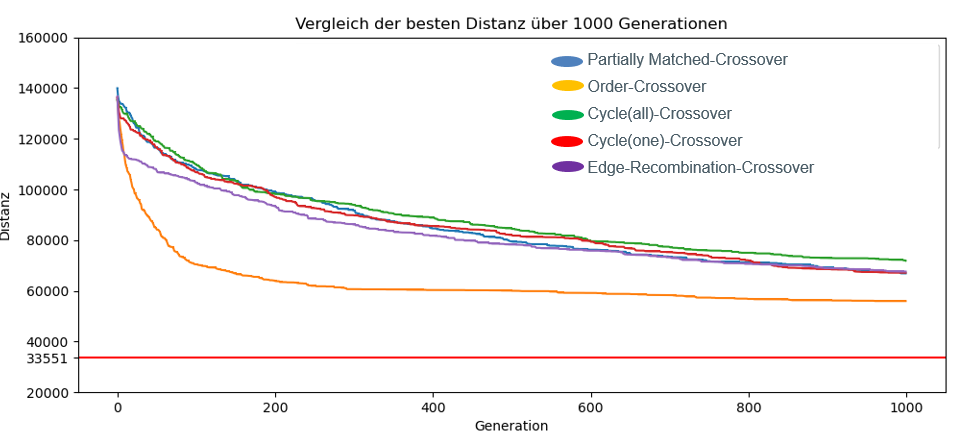
\includegraphics[width=1\textwidth]{img/Vortrag/experiment1.png}
\caption{Ergebnisse des Experiment 1}
\label{fig:experiment1}
\end{figure}

\subsection{Experiment 2}

\begin{figure}[H]
\centering
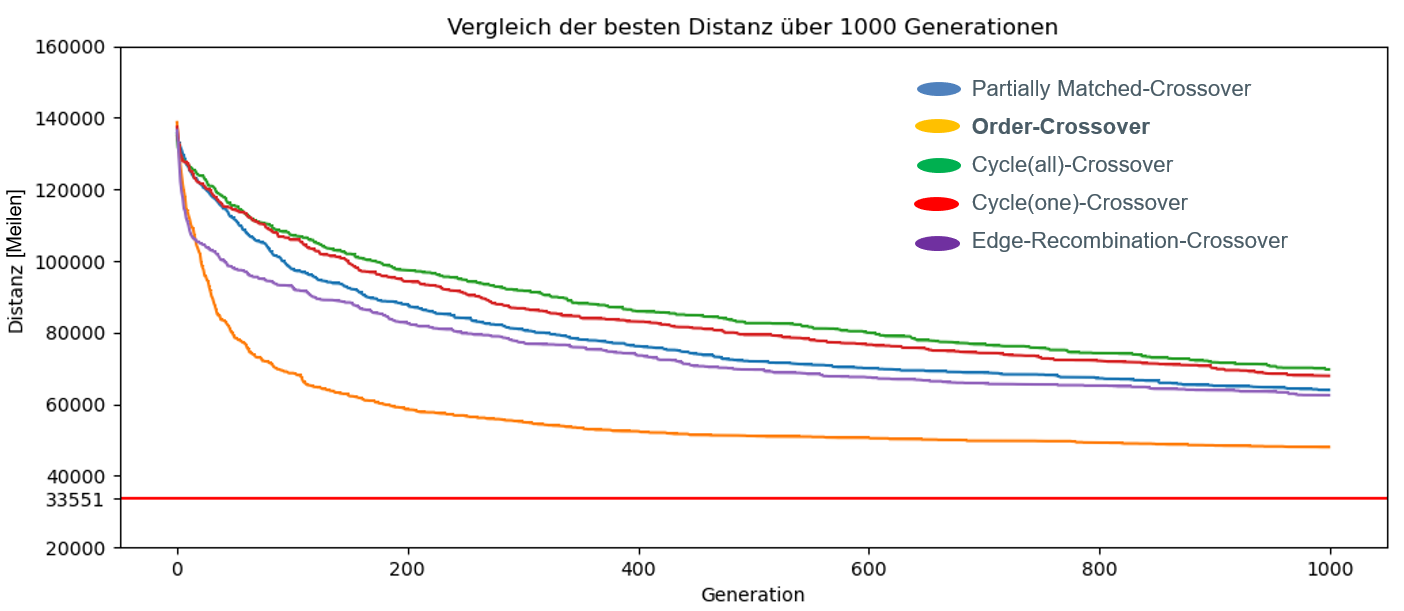
\includegraphics[width=1\textwidth]{img/Vortrag/experiment2.png}
\caption{Ergebnisse des Experiment 2}
\label{fig:experiment2}
\end{figure}

\subsection{Experiment 3}

\begin{figure}[H]
\centering
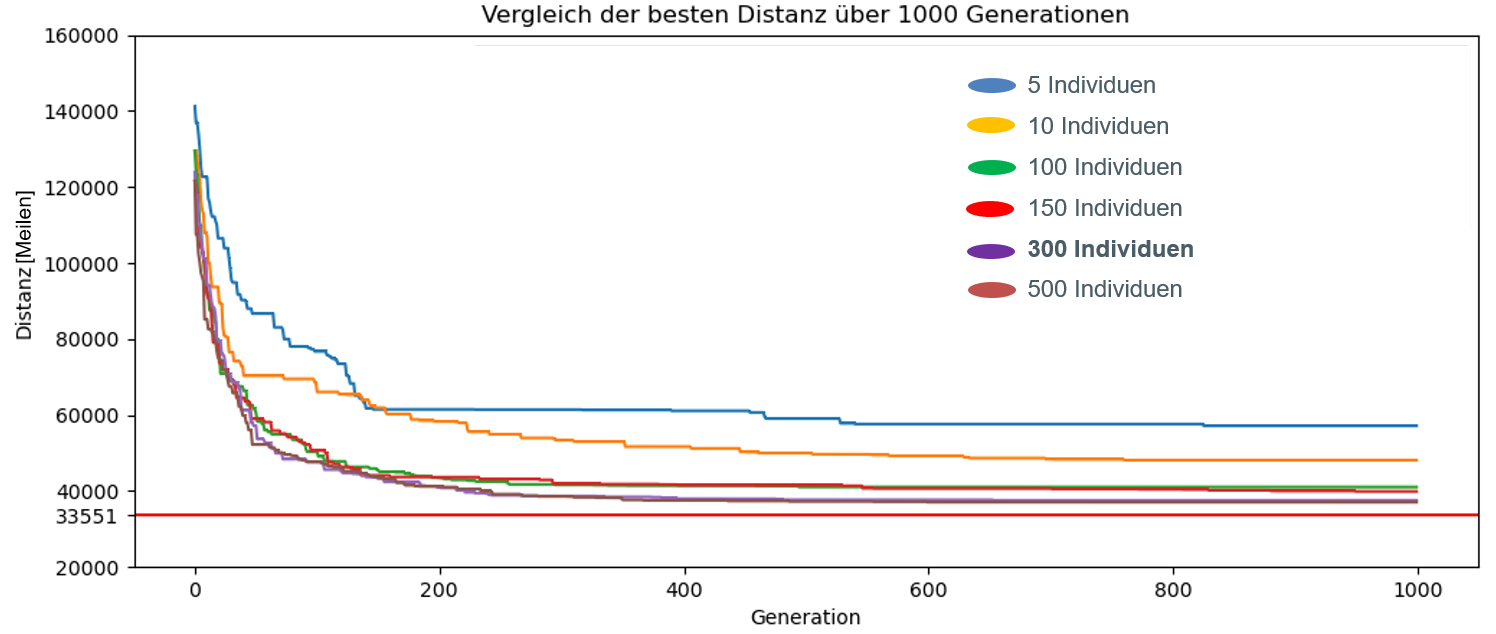
\includegraphics[width=1\textwidth]{img/Vortrag/experiment3.png}
\caption{Ergebnisse des Experiment 3}
\label{fig:experiment3}
\end{figure}

\subsection{Experiment 4}

\begin{figure}[H]
\centering
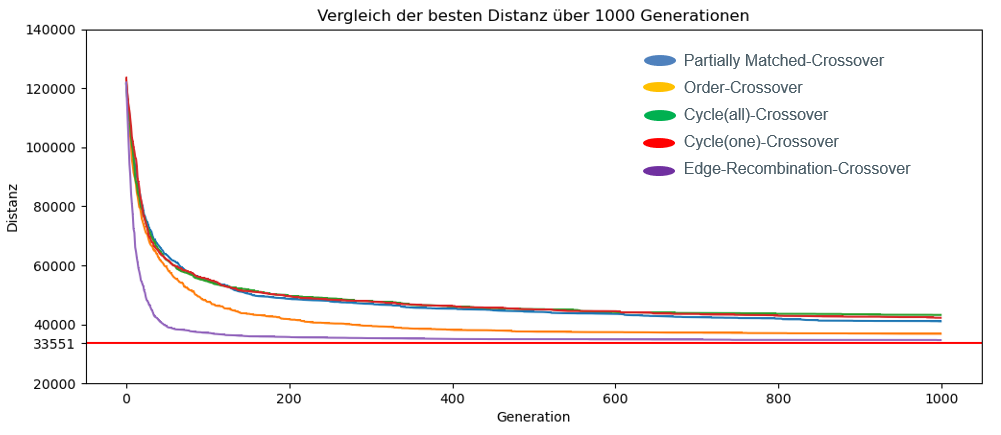
\includegraphics[width=1\textwidth]{img/Vortrag/experiment4.png}
\caption{Ergebnisse des Experiment 4}
\label{fig:experiment4}
\end{figure}

\subsection{Experiment 5}

\begin{figure}[H]
\centering
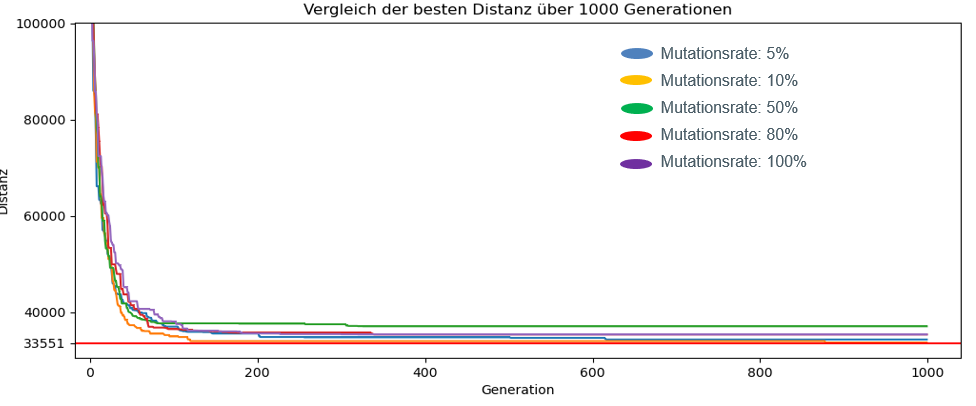
\includegraphics[width=1\textwidth]{img/Vortrag/experiment5.png}
\caption{Ergebnisse des Experiment 5}
\label{fig:experiment5}
\end{figure}

\subsection{Experiment 6}

\begin{figure}[H]
\centering
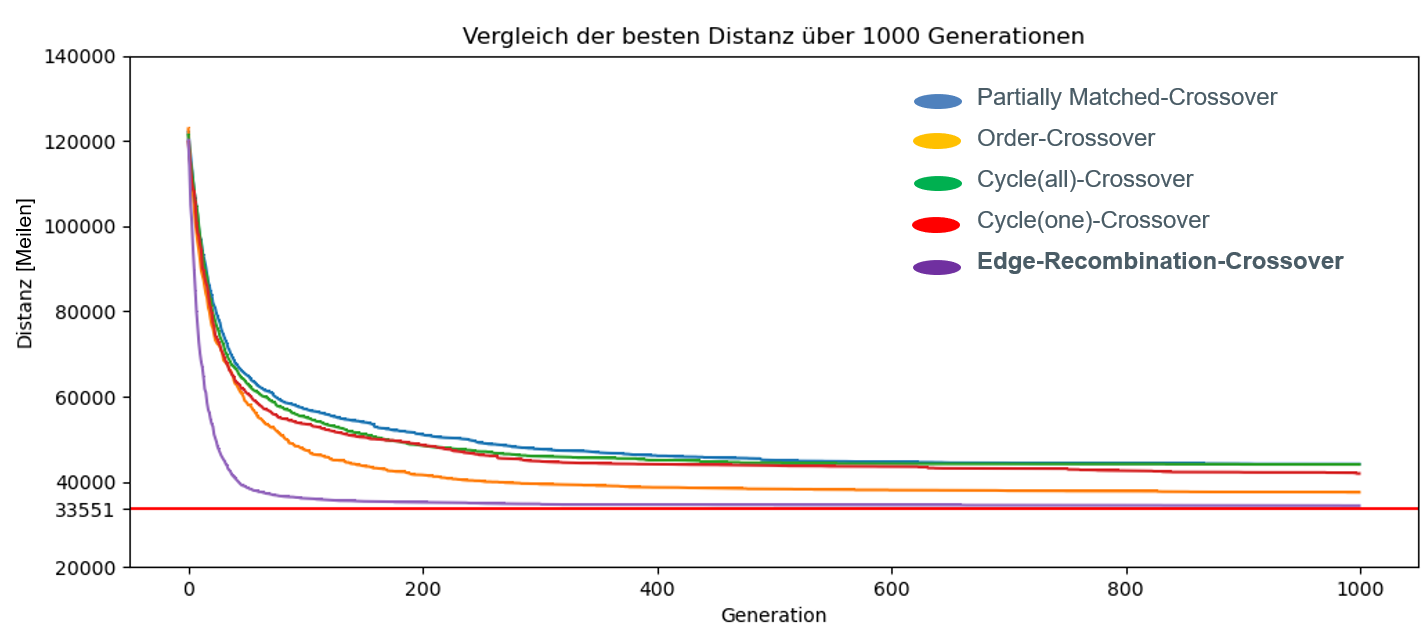
\includegraphics[width=1\textwidth]{img/Vortrag/experiment6.png}
\caption{Ergebnisse des Experiment 6}
\label{fig:experiment6}
\end{figure}

\subsection{Experiment 7}

\begin{figure}[H]
\centering
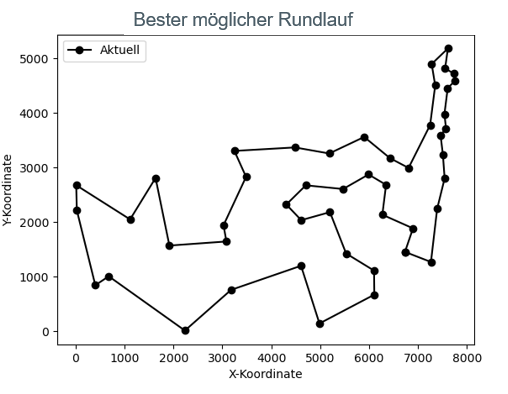
\includegraphics[width=1\textwidth]{img/Vortrag/experiment7_1.png}
\caption{Ergebnisse des Experiment 7.1}
\label{fig:experiment71}
\end{figure}
\begin{figure}[H]
\centering
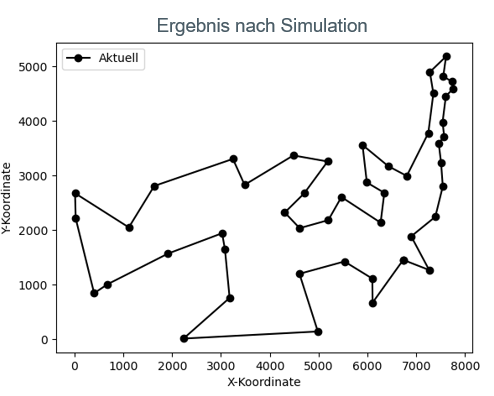
\includegraphics[width=1\textwidth]{img/Vortrag/experiment7_2.png}
\caption{Ergebnisse des Experiment 7.2}
\label{fig:experiment72}
\end{figure}
%--